\documentclass{article}
% % % % % % % % % % % % % % % % % % % 
%
%  USEPACKAGES; kept minimal, these can be ammended but not removed.
%
% % % % % % % % % % % % % % % % % % %
\usepackage{fancyhdr}
\usepackage{pdfpages}
\usepackage{graphicx}
\usepackage{hyperref}
\usepackage[utf8]{inputenc}
\usepackage{longtable}
\usepackage{listings}
\usepackage[acronym]{glossaries}
\usepackage{multirow}
\usepackage{amsmath}
%
% Add other packages here
%

\newcommand{\studentNumber}{M009900X9}
\newcommand{\moduleCode}{CST3590}
\title{\moduleCode: Proposal}
\author{A. N. Onymous\\ \studentNumber}

\begin{document}
\maketitle

\section{Introduction}
Blockchain Technology is the engine behind Web3.0, Decentralisation and predicted to become the next General Purpose Technology \cite{filippova2019empirical}.
Blockchain Technology across a wide spectrum of domains, e.g., Medicine \cite{azaria2016medrec}, Education \cite{mitchell2020blockchain} and Finance \cite{treleaven2017blockchain}.
Consensus algorithms are essential to blockchain technology and are investigated further in the literature review. 

Some of these consensus algorithms are responsible for unsustainability \cite{sutherland2019blockchain}, particularly Proof-of-Work in Bitcoin.
This project aims to propose a consensus algorithm that is sustainable for the future.

\section{Aims }
To design, develop, evaluate, analyse and compare the proposed consensus algorithm with existing consensus algorithms.

\subsection{Objectives}
The project's objectives are as follows:
\begin{enumerate}
	\item Complete design of blockchain system in Python
	\item Complete Proof-of-Elapsed-Time in Python 
	\item Design a consensus algorithm that is Fault Tolerant 
	\item Run varying tests on the proposed algorithm
	\item Evaluate and compare the tests
	\item Analyse the results and tests 
\end{enumerate}

\section{Resources}
To complete this project access to a laptop running a Linux with the following specifications:
\begin{itemize}
	\item Linux Ubuntu 24.04
	\item Node Package Manager
	\item Python3
	\item 16Gb RAM
	\item 256Gb SSD
	\item intel i5 or equivalent
\end{itemize}


\section{Planning}
A GANTT chart is presented in fig. \ref{gantt} and shows the progress of this project over 12 weeks.

\begin{figure}
	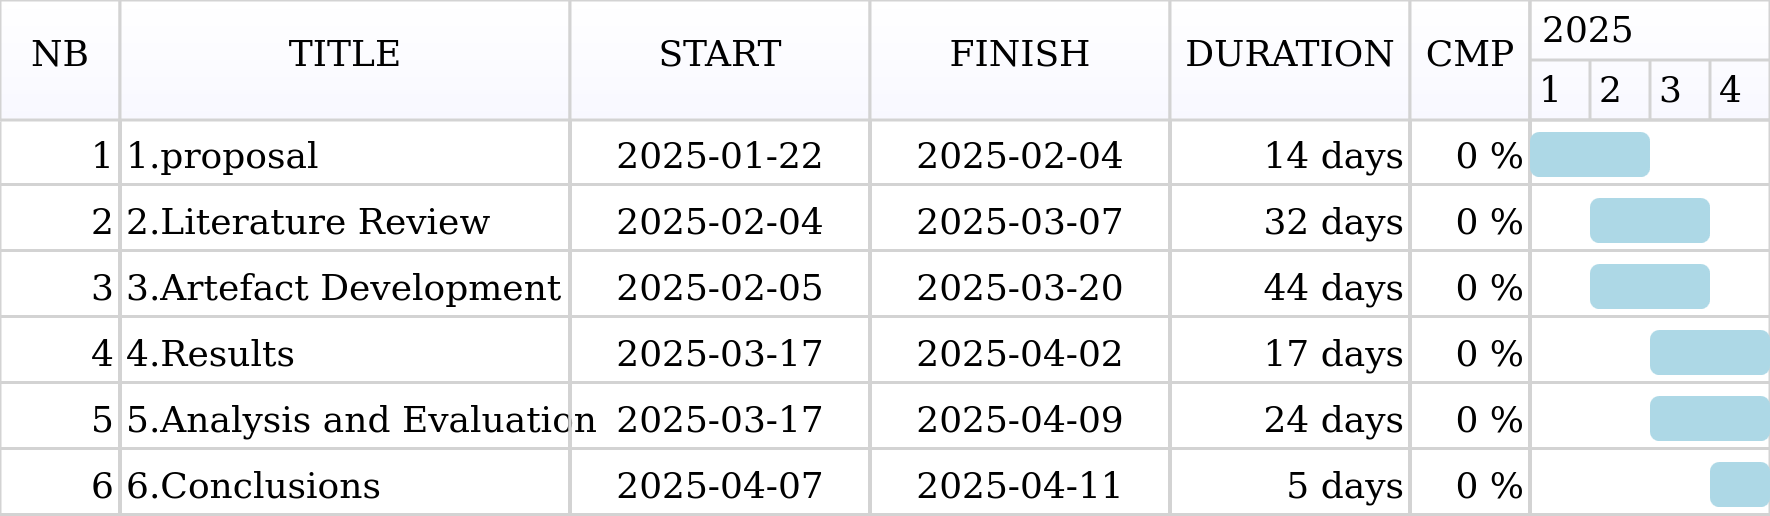
\includegraphics[scale=0.25]{DrawGanttMonth}
	\caption{GANTT chart for individual project}
	\label{gantt}
\end{figure}


\section{Ethics}
This project is considered minimal risk and the ethical review form has been attached in the appendix of this document.


%\bibliographystyle{plain}
\bibliographystyle{IEEEtranS}
\bibliography{references}

\section*{Appendix A}
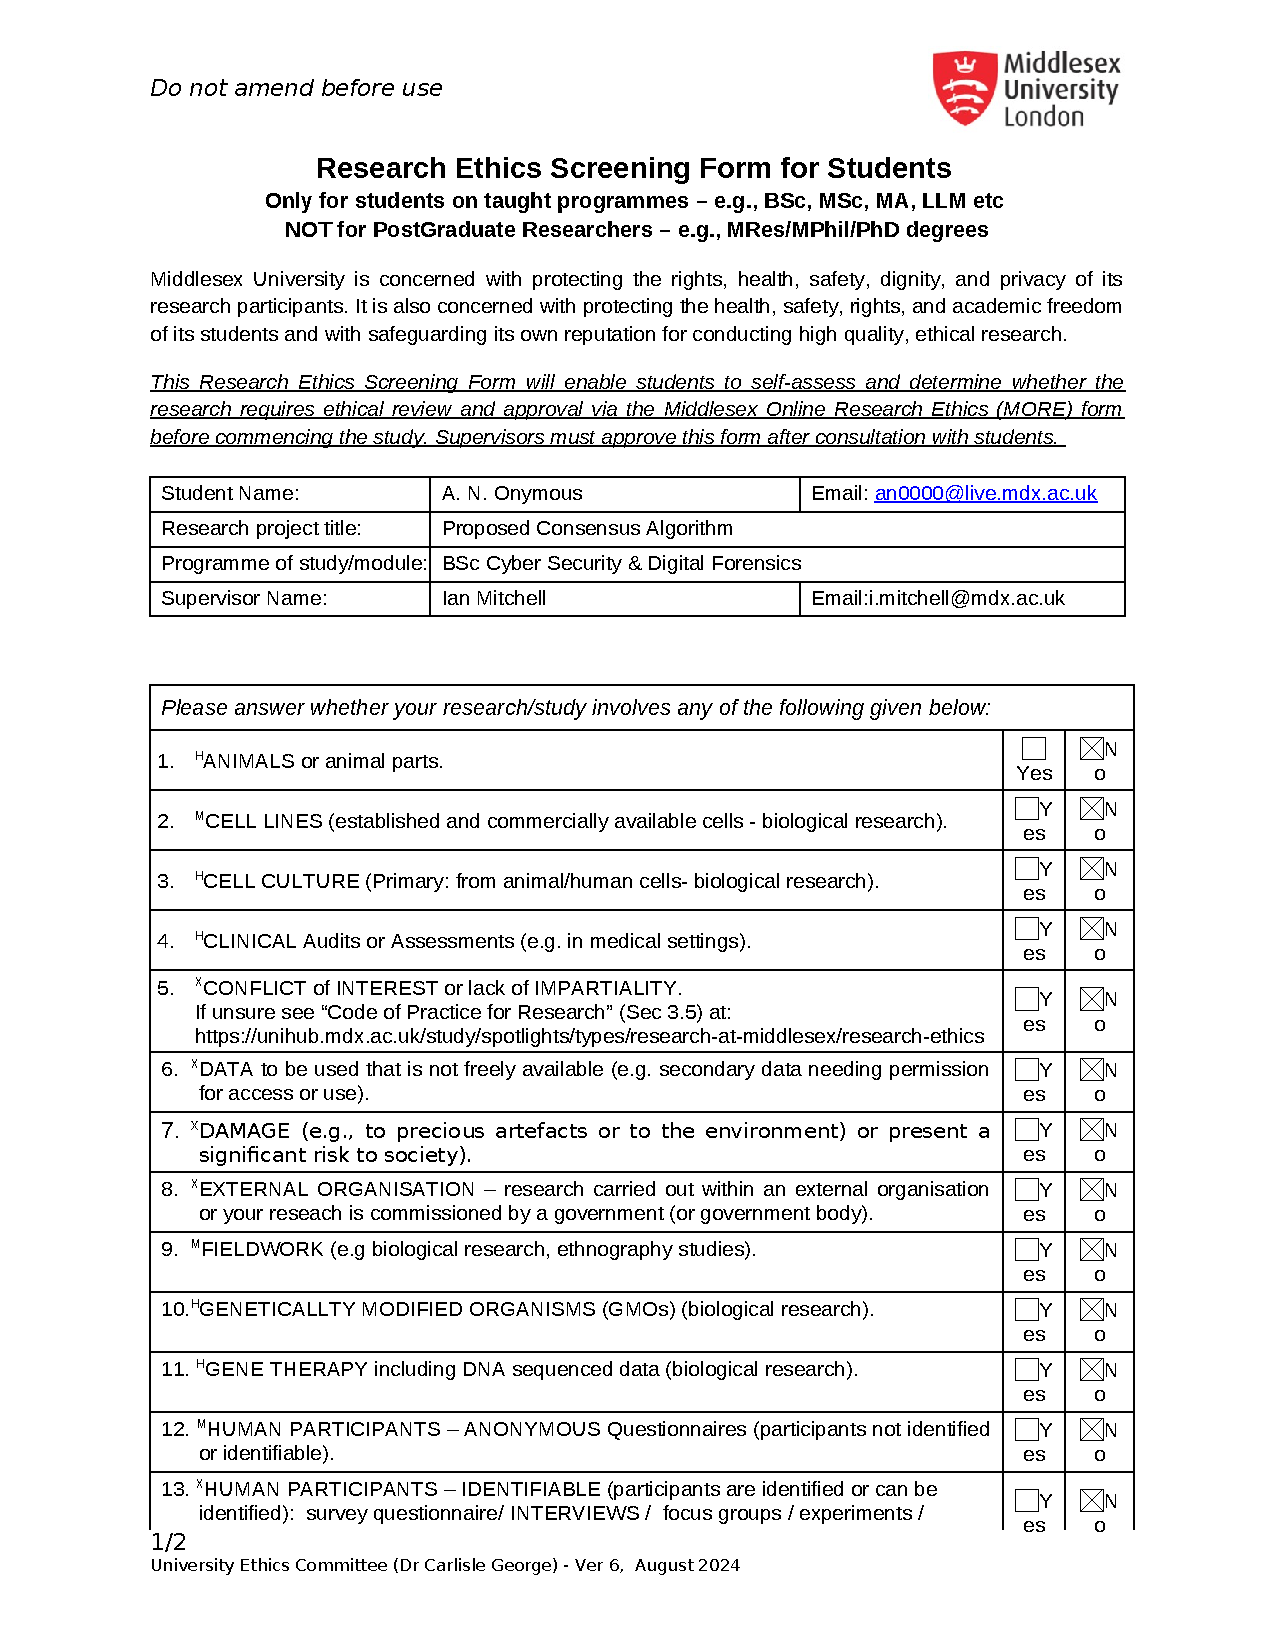
\includepdf[pages=-,scale=0.75]{ethics}


\end{document}
